\chapter{Versuch 3}
\label{chap:VERSUCH_3}

\section{Fragestellung, Messprinzip, Aufbau, Messmittel}
\label{chap:VERSUCH_3_FRAGESTELLUNG}

\subsection*{Fragesetellung}

Die Sensitivität von Kamerasensoren ist aufgrund von Fertigungstoleranzen nicht völlig gleich.
Zudem Kommt es durch das Objectiv der Kamera zu einer sogenannten Vignettierung, d.h. der Rand des Bildes ist dunkler als er sein sollte, weil das Licht ungleichmäßig verteilt wird.
Das beides führt dazu, das einige Pixel einen zu geringen Helligkeitswert aufweisen.
In diesen Versuch geht es darum diese Pixel zu finden und unsere Aufnahmen so zu kalibrieren das diese Pixel kein Problem mehr sind.

\subsection*{Messprinzip}
Wird eine Aufnahme von einen weißen Blatt Papier gemacht heben sich auf dem resultierenden Bild Schatten und zu dunkle Pixel hervor.
So kann man ermitteln welche Pixel einen zu dunklen Wert angeben.
Leider wird das Ergebnis durch starke Lichteinstrahlung und Schatten von außen verfälscht.
Daher ist es wichtig die Beleuchtung gleichmäßig zu halten, die Einflüsse äußeren Faktoren zu minimieren.

\subsection*{Aufbau}

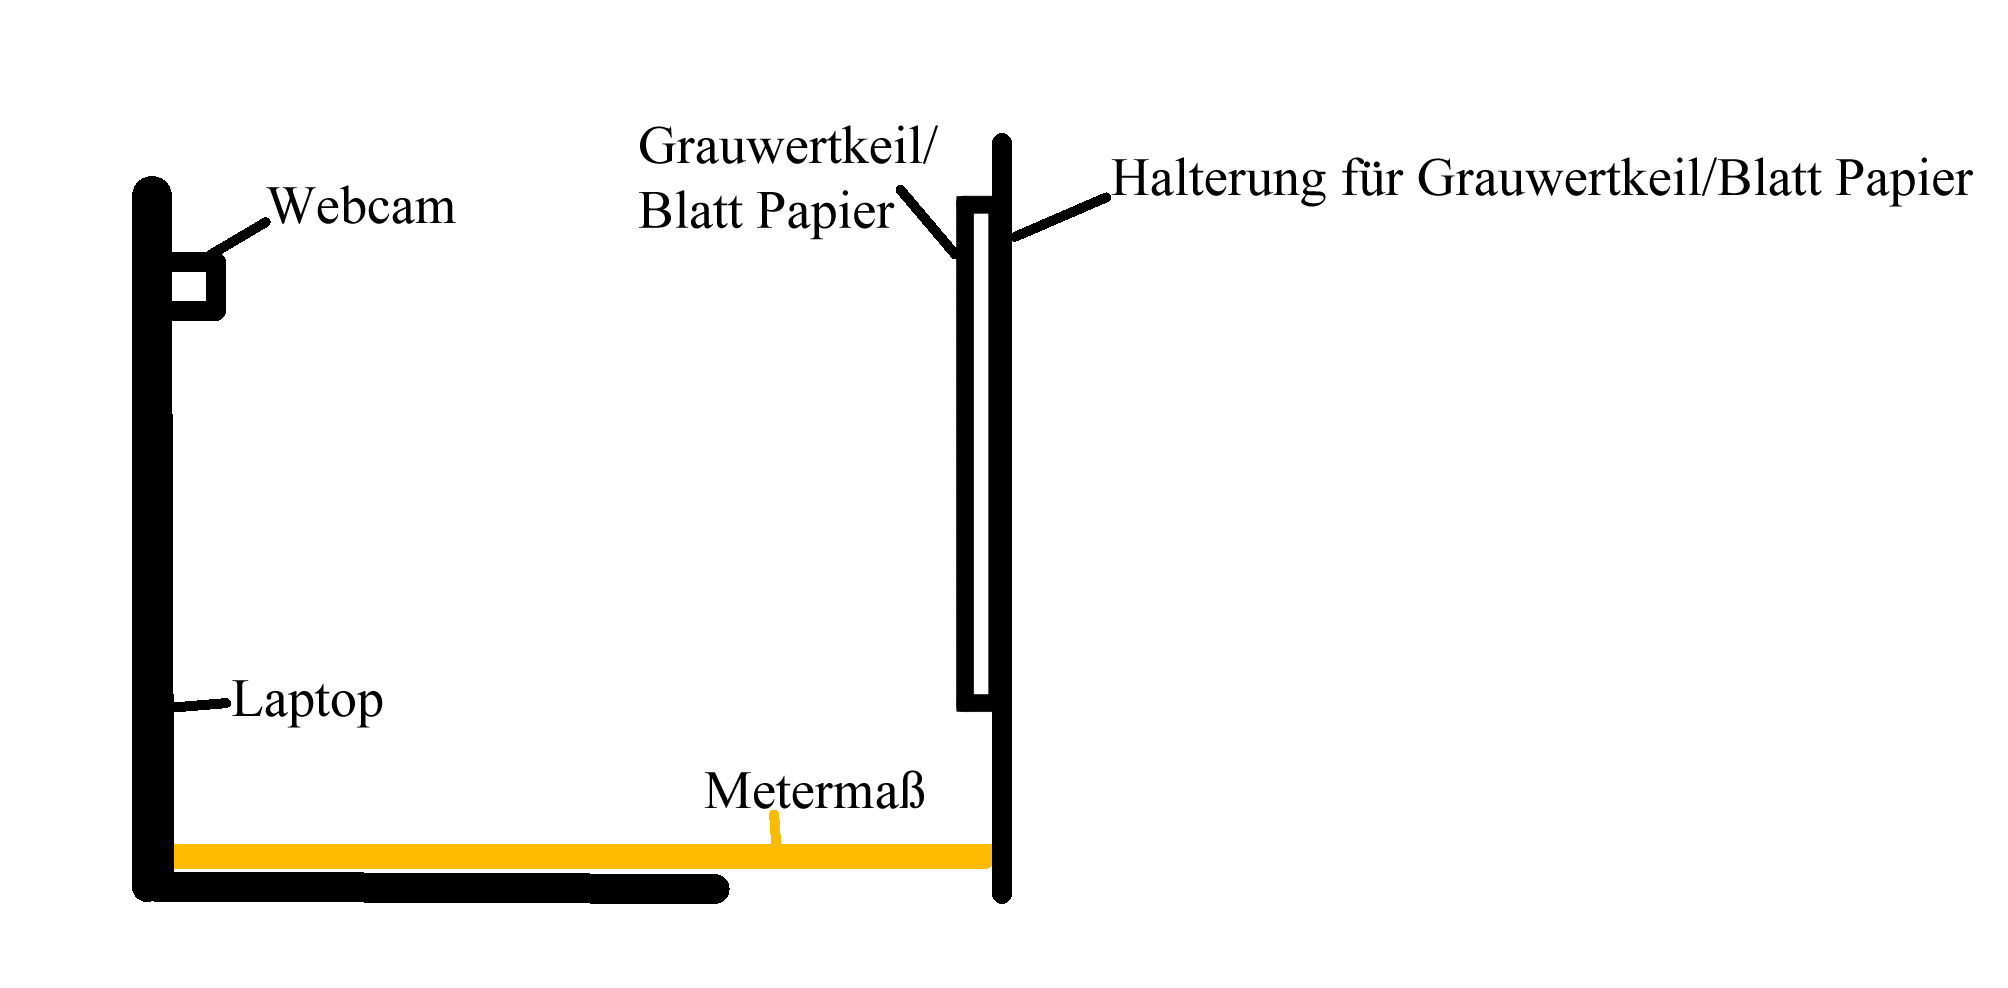
\includegraphics[scale=0.4]{media/Versuchsaufbau_2.png}

\subsection{Messmittel}
\begin{itemize}
\item Webcame (Asus USB2.0 UVC HD Webcam)
\item weißes Blatt Papier
\item Metermaß
\end{itemize}


\section{Messwerte}
\label{chap:VERSUCH_3_MESSWERTE}

\begin{tabular}{c c c c c}

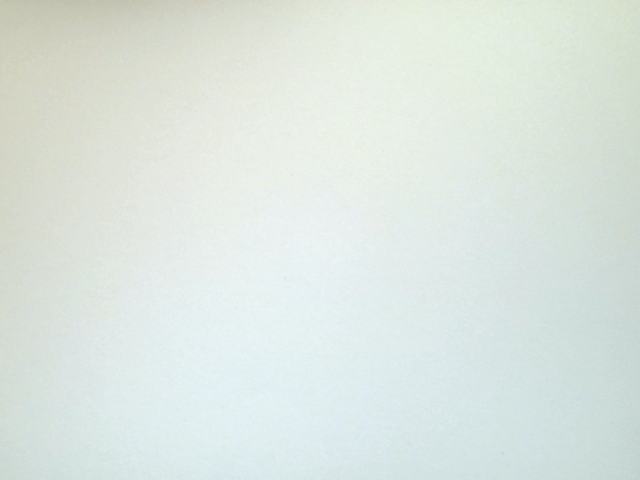
\includegraphics[scale=0.11]{media/weissbilder/weissbild_0.png}
 & 

\includegraphics[scale=0.11]{media/weissbilder/weissbild_1.png}
 &

\includegraphics[scale=0.11]{media/weissbilder/weissbild_2.png}
 & 

\includegraphics[scale=0.11]{media/weissbilder/weissbild_3.png}
 &

\includegraphics[scale=0.11]{media/weissbilder/weissbild_4.png}
 \\ 

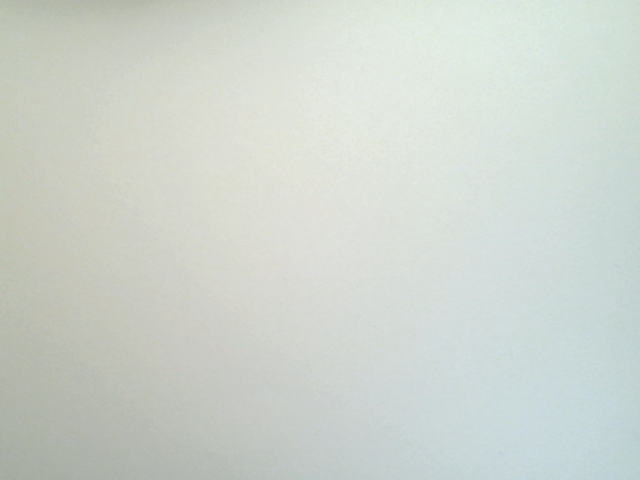
\includegraphics[scale=0.11]{media/weissbilder/weissbild_5.png}
 & 

\includegraphics[scale=0.11]{media/weissbilder/weissbild_6.png}
 & 

\includegraphics[scale=0.11]{media/weissbilder/weissbild_7.png}
 &

\includegraphics[scale=0.11]{media/weissbilder/weissbild_8.png}
 & 

\includegraphics[scale=0.11]{media/weissbilder/weissbild_9.png}
\end{tabular} 
\captionof{figure}{Fig: Weißbilder Nr. 0-9}

\section{Auswertung}
\label{chap:VERSUCH_3_AUSWERTUNG}

zur Auswertung des Weißbildes wird zunächst der Mittelwert der zehn Weißbilder erstellt, d.h. es soll ein künstliches Weißbild erstellt werden, bei den jeder Pixel der Mittelwert der entsprechenden Pixel der anderen Weißbilder ist.

\subsection*{Mittelwertbild des Weißbildes}
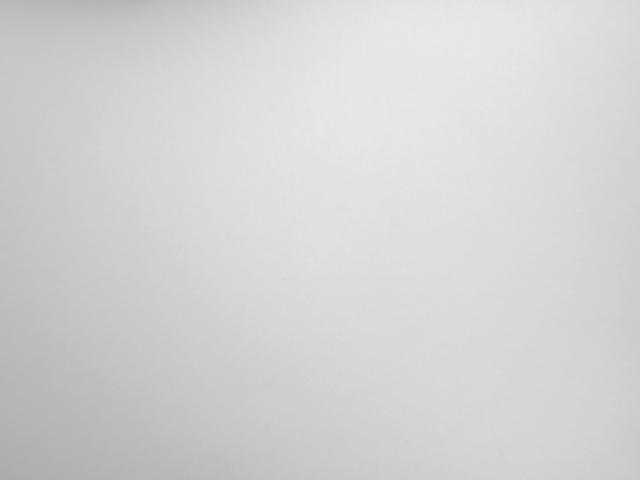
\includegraphics[scale=0.6]{media/weissMean.png}
\captionof{figure}{Fig: Mittelwertbild der Weißbilder}

Um die Deadpixel und die Vignettierung zu verdeutlichen wurde das Mittelwertweißbild noch kontrastmaximiert. Das kontrastmaximiete Bild dient nur zur Veranschaulichung und ist für weitere Auswertungen irrelevant.

\subsection*{Kontrastmaximiertes Weißbild}
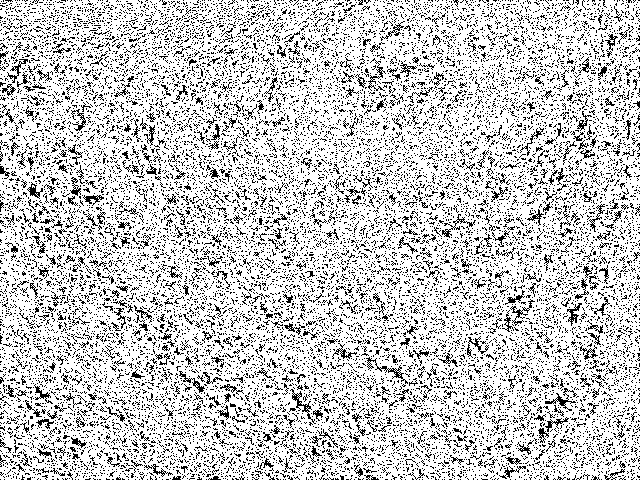
\includegraphics[scale=0.6]{media/weissContrastMax.png}
\captionof{figure}{Fig: Kontrastmaximiertes Weißbild}

\section{Interpretation}
\label{chap:VERSUCH_3_INTERPRETATION}

Das Kontrastmaximierte Bild zeigt, dass vor allen die linken Ecken des Bildes viele verdunkelte Pixel haben. Das deckt sich mit den Aufnahmen selbst, bei welchen auch ohne erhöhten Kontrast ein Schatten in der linken unteren Ecke auffällt.
Zudem ist das Bild oben mittig am hellsten.
Dieser Schattenunterschied ist vermutlich mehr durch äußere Beleuchtungsbedingungen zu erklären als durch die Deadpixel und  die Vignettierung. Es sei hierbei erwähnt das die Aufnahmen nach Einbruch der Dunkelheit gemacht wurden und die Lichtquelle eine Deckenbeleuchtung war.

Dennoch kann man erkennen, das der Rand dunkler ist als der Rand generell dunkler ist, die Effekte der Vignettierung wurden also erfasst.
Und auch die Deadpixel lassen sich erkennen, da es selbst in den Hellen Teilen vereinzelte dunkle Flecken gibt.
